
\section*{\LARGE{Appendix}}
\vspace{-1ex}
\section{Results on Soft Filter Pruning \citep{he2018sfp}}
\label{sec:sfp}


\textbf{Soft Filter Pruning (SFP) \citep{he2018sfp}} prunes filters every epoch during training but also keeps updating the pruned filters, i.e., the pruned weights have the chance to be recovered. In the original paper, SFP can either run upon a random initialized model or a pretrained model. It falls into the category of predefined methods (\autoref{auto}). \autoref{sfp-1} shows our results without using pretrained models and \autoref{sfp-2} shows the results with a pretrained model. We use authors' code \citep{sfpcode} for obtaining the results. It can be seen that Scratch-E outperforms pruned models for most of the time and Scratch-B outperforms pruned models in nearly all cases. Therefore, our observation also holds on this method.

\setlength{\tabcolsep}{4pt}
\renewcommand{\arraystretch}{1.25}
\begin{table}[!htbp]
% \vspace{-1ex}
\centering
\small
\resizebox{0.98\textwidth}{!}{
\begin{tabular}{c|c|ccccc}
\hline
Dataset                    & Model                       & Unpruned             & Prune Ratio & Pruned      & Scratch-E   & Scratch-B   \\ \hline
\multirow{13}{*}{CIFAR-10} & \multirow{3}{*}{ResNet-20}  &   \multirow{3}{*}{92.41 ($\pm$0.12)}                    & 10\%        & 92.00 ($\pm$0.32) & \textbf{92.22} ($\pm$0.15) & 92.13 ($\pm$0.10) \\
                           &                            &                      & 20\%        & 91.50 ($\pm$0.30) & 91.62 ($\pm$0.12) & \textbf{91.67} ($\pm$0.15) \\
                           &                             &                      & 30\%        & 90.78 ($\pm$0.15) & 90.93 ($\pm$0.10) & \textbf{91.07} ($\pm$0.23) \\ \cline{2-7} 
                           & \multirow{3}{*}{ResNet-32}  &   \multirow{3}{*}{93.22 ($\pm$0.16)}                    & 10\%        & 93.28 ($\pm$0.05) & \textbf{93.42} ($\pm$0.40) & 93.08 ($\pm$0.13) \\
                           &                             &                      & 20\%        & 92.50 ($\pm$0.17) & 92.68 ($\pm$0.20) & \textbf{92.96} ($\pm$0.11) \\
                           &                             &                      & 30\%        & 92.02 ($\pm$0.11) & 92.37 ($\pm$0.12) & \textbf{92.56} ($\pm$0.06) \\ \cline{2-7} 
                           & \multirow{4}{*}{ResNet-56}  &    \multirow{4}{*}{93.80 ($\pm$0.12)}                   & 10\%        & 93.77 ($\pm$0.07) & 93.42 ($\pm$0.40) & \textbf{93.98} ($\pm$0.21) \\
                           &                             & \multicolumn{1}{l}{} & 20\%        & 93.14 ($\pm$0.42) & 93.44 ($\pm$0.05) & \textbf{93.71} ($\pm$0.14) \\
                           &                             & \multicolumn{1}{l}{} & 30\%        & 93.01 ($\pm$0.09) & 93.19 ($\pm$0.20) & \textbf{93.57} ($\pm$0.12) \\
                           &                             & \multicolumn{1}{l}{} & 40\%        & 92.59 ($\pm$0.14) & 92.80 ($\pm$0.25) & \textbf{93.07} ($\pm$0.25) \\ \cline{2-7} 
                           & \multirow{3}{*}{ResNet-110} & \multirow{3}{*}{93.77 ($\pm$0.23)}  & 10\%        & 93.60 ($\pm$0.50) & \textbf{94.21} ($\pm$0.39) & 94.13 ($\pm$0.37) \\
                           &                             & \multicolumn{1}{l}{} & 20\%        & 93.63 ($\pm$0.44) & 93.52 ($\pm$0.18) & \textbf{94.29} ($\pm$0.18) \\
                           &                             & \multicolumn{1}{l}{} & 30\%        & 93.26 ($\pm$0.37) & 93.70 ($\pm$0.16) & \textbf{93.92} ($\pm$0.13) \\ \hline
\multirow{2}{*}{ImageNet}  & ResNet-34                   & 73.92                & 30\%        & 71.83       & 71.67       & \textbf{72.97}       \\ \cline{2-7} 
                           & ResNet-50                   & 76.15                & 30\%        & 74.61       & 74.98       & \textbf{75.56}       \\ \hline
\end{tabular}
}
\vspace{2ex}
\caption{Results (accuracy) for Soft Filter Pruning \citep{he2018sfp} without pretrained models.}
\label{sfp-1}
% \vspace{-4ex}
\end{table}

\setlength{\tabcolsep}{4pt}
\renewcommand{\arraystretch}{1.25}
\begin{table}[!htbp]
\vspace{-1ex}
\centering
\small
\resizebox{\textwidth}{!}{
\begin{tabular}{c|c|ccccc}
\hline
Dataset                   & Model                      & Unpruned & Prune Ratio & Pruned      & Scratch-E   & Scratch-B   \\ \hline
\multirow{3}{*}{CIFAR-10} & \multirow{2}{*}{ResNet-56} &    \multirow{2}{*}{93.80 ($\pm$0.12)}       & 30\%        & 93.51 ($\pm$0.26) & \textbf{94.45} ($\pm$0.30) & 93.77 ($\pm$0.25) \\
                          &                            &          & 40\%        & 93.10 ($\pm$0.34) & \textbf{93.84} ($\pm$0.16) & 93.41 ($\pm$0.08) \\ \cline{2-7} 
                          & ResNet-110                 &   \multirow{1}{*}{93.77 ($\pm$0.23)}       & 30\%        & 93.46 ($\pm$0.19) & 93.89 ($\pm$0.17) & \textbf{94.37} ($\pm$0.24) \\ \hline
\end{tabular}
}
\vspace{2ex}
\caption{Results (accuracy) for Soft Filter Pruning \citep{he2018sfp} using pretrained models.}
\label{sfp-2}
% \vspace{-4ex}
\end{table}




\section{Transfer Learning to Object Detection}
\label{sec:transfer}

We have shown that for structured pruning the small pruned model can be trained from scratch to match the accuracy of the fine-tuned model in classification tasks. To see whether this phenomenon would also hold for transfer learning to other vision tasks, we evaluate the $L_1$-norm based filter pruning method \citep{li2016pruning} on the PASCAL VOC object detection task, using Faster-RCNN \citep{ren2015faster}. 
\vspace{-1ex}

Object detection frameworks usually require transferring model weights pre-trained on ImageNet classification, and one can perform pruning either before or after the weight transfer. More specifically, the former could be described as ``train on classification, prune on classification, fine-tune on classification, transfer to detection'', while the latter is ``train on classification, transfer to detection, prune on detection, fine-tune on detection''. We call these two approaches Prune-C (classification) and Prune-D (detection) respectively, and report the results in \autoref{det-prune}. With a slight abuse of notation, here Scratch-E/B denotes "train the small model on classification, transfer to detection", and is different from the setup of detection without ImageNet pre-training as in \cite{dsod}.

\begin{table}[ht]
\begin{minipage}{\linewidth}
% \vspace{2ex}
\centering
\small
% \renewcommand{\arraystretch}{1.4}
% \setlength{\tabcolsep}{1.4pt}
\resizebox{1.0\textwidth}{!}{
\begin{tabular}{l|l|c|ccccc}
\hline
\multicolumn{1}{c|}{Dataset}   & \multicolumn{1}{c|}{Model} & \multicolumn{1}{c|}{Unpruned} & Pruned Model & Prune-C & Prune-D & Scratch-E & Scratch-B                        \\ \hline
\multirow{2}{*}{PASCAL VOC 07} & \multirow{2}{*}{ResNet-34} & \multirow{2}{*}{71.69}       & ResNet34-A   & 71.47   & 70.99   & 71.64 & \textbf{71.90}\\ \cline{4-8} 
                               &                            &                              & ResNet34-B   & 70.84   & 69.62   & \textbf{71.68}  & 71.26 \\ \hline
\end{tabular}
}
\vspace{2ex}
\captionof{table}{Results (mAP) for pruning on detection task. The pruned models are chosen from \citet{li2016pruning}. Prune-C refers to pruning on classifcation pre-trained weights, Prune-D refers to pruning after the weights are transferred to detection task. Scratch-E/B means pre-training the pruned model from scratch on classification and transfer to detection.}
\label{det-prune}
\end{minipage}\hfill
\vspace{-4ex}
\end{table}

For this experiment, we adopt the code and default hyper-parameters from \cite{jjfaster2rcnn}, and use PASCAL VOC 07 trainval/test set as our training/test set. For backbone networks, we evaluate ResNet-34-A and ResNet-34-B from the $L_1$-norm based filter pruning \citep{li2016pruning}, which are pruned from ResNet-34.
\autoref{det-prune} shows our result, and we can see that the model trained from scratch can surpass the performance of fine-tuned models under the transfer setting.
\vspace{-1ex}

Another interesting observation from \autoref{det-prune} is that Prune-C is able to outperform Prune-D, which is surprising since if our goal task is detection, directly pruning away weights that are considered unimportant for detection should presumably be better than pruning on the pre-trained classification models. We hypothesize that this might be because pruning early in the classification stage makes the final model less prone to being trapped in a bad local minimum caused by inheriting weights from the large model. This is in line with our observation that Scratch-E/B, which trains the small models from scratch starting even earlier at the classification stage, can achieve further performance improvement.

\section{Aggressively Pruned Models}

It would be interesting to see whether our observation still holds if the model is very aggressively pruned, since they might not have enough capacity to be trained from scratch and achieve decent accuracy. Here we provide results using Network Slimming \citep{liu2017learning} and $L_1$-norm based filter pruning~\citep{li2016pruning}.  From \autoref{significant}, \autoref{significant-2} and \autoref{significant-3}, it can be seen that when the prune ratio is large, training from scratch is better than fine-tuned models by an even larger margin, and in this case fine-tuned models are significantly worse than the unpruned models. Note that in \autoref{thinet}, the VGG-Tiny model we evaluated for ThiNet \citep{luo2017thinet} is also a very aggressively pruned model (FLOPs reduced by 15$\times$ and parameters reduced by 100$\times$).
\setlength{\tabcolsep}{4pt}
\renewcommand{\arraystretch}{1.15}
\begin{table}[!htbp]
\vspace{-1ex}
\centering
\small
% Please add the following required packages to your document preamble:
% \usepackage{multirow}
\resizebox{\textwidth}{!}{
\begin{tabular}{c|c|ccccc}
\hline
Dataset                   & Model                          & Unpruned                           & Prune Ratio & Fine-tuned        & Scratch-E         & Scratch-B                                   \\ \hline
\multirow{4}{*}{CIFAR-10} & PreResNet-56                   & 93.69 ($\pm$0.07)                  & 80\%       & 74.66 ($\pm$0.96) & 88.25 ($\pm$0.38) & \textbf{88.65} ($\pm$0.32)                           \\ \cline{2-7} 
                          & \multirow{2}{*}{PreResNet-164} & \multirow{2}{*}{95.04 ($\pm$0.16)} & 80\%        & 91.76 ($\pm$0.38) & 93.21 ($\pm$0.17) & \textbf{93.49} ($\pm$0.20) \\
                          &                                &                                    & 90\%        & 82.06 ($\pm$0.92) & 87.55 ($\pm$0.68) & \textbf{88.44} ($\pm$0.19) \\ \cline{2-7} 
                          & DenseNet-40                    & 94.10 ($\pm$0.12)                  & 80\%        & 92.64 ($\pm$0.12) & 93.07 ($\pm$0.08) & \textbf{93.61} ($\pm$0.12) \\ \hline
CIFAR-100                 & DenseNet-40                    & 73.82 ($\pm$0.34)                  & 80\%        & 69.60 ($\pm$0.22) & 71.04 ($\pm$0.36) & \textbf{71.45} ($\pm$0.30) \\ \hline
\end{tabular}
}
\vspace{2ex}
\caption{Results (accuracy) for Network Slimming~\citep{liu2017learning} when the models are aggressively pruned. ``Prune ratio'' stands for total percentage of channels that are pruned in the whole network. Larger ratios are used than the original paper of \citet{liu2017learning}. 
}
\label{significant}
\end{table}



\renewcommand{\arraystretch}{1.15}
\begin{table}[!htbp]
\small
\vspace{-2ex}
\centering
\resizebox{1.0\textwidth}{!}{
\begin{tabular}{c|c|cccccc}
\hline
Dataset                   & Model                       & Unpruned                                               & Prune Ratio & Fine-tuned                             & Scratch-E                                   & \multicolumn{1}{c}{Scratch-B}   \\ \hline
\multirow{1}{*}{CIFAR-10} & ResNet-56                      & 93.14 ($\pm$0.12)  & 90\%   & 89.17 ($\pm$0.08)  & 91.02 ($\pm$0.12) & \textbf{91.93} ($\pm$0.26)                           \\ \hline
\end{tabular}
}
\vspace{1ex}
\caption{Results (accuracy) for $L_1$-norm based filter pruning \citep{li2016pruning} when the models are aggressively pruned.
}
\label{significant-2}
\vspace{-2ex}
\end{table}

\renewcommand{\arraystretch}{1.15}
\begin{table}[!htbp]
\small
\vspace{-2ex}
\centering
\resizebox{1.0\textwidth}{!}{
\begin{tabular}{c|c|cccccc}
\hline
Dataset                   & Model                       & Unpruned                                               & Prune Ratio & Fine-tuned                             & Scratch-E                                   & \multicolumn{1}{c}{Scratch-B}   \\ \hline
\multirow{1}{*}{CIFAR-10} & VGG-19                      & 93.50 ($\pm$0.11)  & 95\%   & 93.34 ($\pm$0.13)  & 93.21 ($\pm$0.17) & \textbf{93.63} ($\pm$0.18)                           \\\cline{1-7}
\multirow{1}{*}{CIFAR-100} & VGG-19                      & 71.70 ($\pm$0.31)  & 95\%   & 70.22 ($\pm$0.38)  & 70.88 ($\pm$0.35) & \textbf{72.08} ($\pm$0.15)                           \\
\hline
\end{tabular}
}
\vspace{1ex}
\caption{Results (accuracy) for unstructured  pruning \citep{han2015learning} when the models are aggressively pruned.
}
\label{significant-3}
\vspace{-3ex}
\end{table}
\vspace{-2ex}

\section{Extending Fine-tuning Epochs}
Generally, pruning algorithms  use fewer epochs for fine-tuning than training the large model \citep{li2016pruning,he2017channel,luo2017thinet}. For example, $L_1$-norm based filter pruning \citep{li2016pruning} uses 164 epochs for training on CIFAR-10 datasets, and only fine-tunes the pruned networks for 40 epochs. This is due to that mostly small learning rates are used for fine-tuning to better preserve the weights from the large model.
Here we experiment with fine-tuning for more epochs (e.g., for the same number of epochs as Scratch-E) and show it does not bring noticeable performance improvement. 

\setlength{\tabcolsep}{5pt}
\renewcommand{\arraystretch}{1.2}
\begin{table}[!htbp]
\small
\centering
\resizebox{1.0\textwidth}{!}{
\begin{tabular}{c|c|ccccc}
\hline
Dataset                   & Model                                                                  & Pruned Model & Fine-tune-40                                  & Fine-tune-80                                   & \multicolumn{1}{c}{Fine-tune-160} &  Scratch-E\\ \hline
\multirow{5}{*}{CIFAR-10} & VGG-16                                                        & VGG-16-A     & 93.40 ($\pm$0.12)                           & 93.45 ($\pm$0.06) &    93.45 ($\pm$0.08)      &   \textbf{93.62} ($\pm$0.11)                \\ \cline{2-7}    & \multirow{2}{*}{ResNet-56}
                           & ResNet-56-A  & \textbf{92.97}
                          ($\pm$0.17) & 92.92 ($\pm$0.15)             & 92.94 ($\pm$0.16)  & 92.96 ($\pm$0.26)    \\
                          &                                                       & ResNet-56-B  & 92.68 ($\pm$0.19) & 92.67 ($\pm$0.14)     &  \textbf{92.76} ($\pm$0.16)  &  92.54 ($\pm$0.19)                         \\ \cline{2-7} 
                          & \multirow{2}{*}{ResNet-110}                      & ResNet-110-A & 93.14 ($\pm$0.16)                           & 93.12 ($\pm$0.19) &     93.04 ($\pm$0.22)    &    \textbf{93.25} ($\pm$0.29)                  \\
                          &                            & ResNet-110-B & 92.69 ($\pm$0.09)                           & 92.75 ($\pm$0.15) &  92.76 ($\pm$0.16)     &  \textbf{92.89} ($\pm$0.43)                      \\ \hline
\end{tabular}
}
\vspace{1ex}
\caption{``Fine-tune-40'' stands for fine-tuning 40 epochs and so on. Scratch-E models are trained for 160 epochs. We observe that fine-tuning for more epochs does not help improve the accuracy much, and models trained from scratch can still perform on par with fine-tuned models.
}
\label{finetune-more}
\vspace{-3ex}
\end{table}
% \vspace{-2ex}
We use $L_1$-norm filter pruning \citep{li2016pruning} for this experiment. \autoref{finetune-more} shows our results with different number of epochs for fine-tuning. It can be seen that fine-tuning for more epochs gives negligible accuracy increase and sometimes small decrease, and Scratch-E models are still on par with models fine-tuned for enough epochs.
% \vspace{-2ex}




\section{Extending the standard training schedule}
In our experiments, we use the standard training schedule for both CIFAR (160 epochs) and ImageNet (90 epochs). Here we show that our observation still holds after we extend the standard training schedule. We use $L_1$-norm based filter pruning~\citep{li2016pruning} for this experiment. \autoref{enough-epochs} shows our results when we extend the standard training schedule of CIFAR from 160 to 300 epochs. We observe that scratch trained models still perform at least on par with fine-tuned models.

\setlength{\tabcolsep}{5pt}
\renewcommand{\arraystretch}{1.2}
\begin{table}[!htbp]
\small
% \vspace{-2ex}
\centering
\resizebox{1.0\textwidth}{!}{
\begin{tabular}{c|c|ccccc}
\hline
Dataset                   & Model                       & Unpruned                     & Pruned Model & Fine-tuned  & Scratch-E   & Scratch-B   \\ \hline
\multirow{5}{*}{CIFAR-10} & \multirow{1}{*}{VGG-16} & \multirow{1}{*}{93.79 ($\pm$0.05)} & VGG-16-A & 93.67 ($\pm$0.11) & 93.74 ($\pm$0.14) & \textbf{93.80} ($\pm$0.09) \\ \cline{2-7}  & \multirow{2}{*}{ResNet-56} & \multirow{2}{*}{93.52 ($\pm$0.05)} & ResNet-56-A & 93.44 ($\pm$0.15) & 93.34 ($\pm$0.17) & \textbf{93.56} ($\pm$0.09) \\
                          &                             &                              & ResNet-56-B & 93.12 ($\pm$0.20) & 93.14 ($\pm$0.21) & \textbf{93.30} ($\pm$0.17) \\ \cline{2-7} & \multirow{2}{*}{ResNet-110} & \multirow{2}{*}{93.82 ($\pm$0.32)} & ResNet-110-A & 93.75 ($\pm$0.24) & 93.80 ($\pm$0.15) & \textbf{94.10} ($\pm$0.12) \\ 
                          &                             &                              & ResNet-110-B & 93.36 ($\pm$0.28) & 93.75 ($\pm$0.16) & \textbf{93.90} ($\pm$0.17) \\ \hline
\end{tabular}
}
\vspace{1ex}
\caption{Results for $L_1$-norm filter pruning~\citep{li2016pruning} when the training schedule of the large model is extended from 160 to 300 epochs.
}
\label{enough-epochs}
\vspace{-3ex}
\end{table}


\section{Weight Distributions}
\label{sec:dist}
\begin{figure}[!htbp]
\centering
\begin{minipage}{\textwidth}
 \begin{subfigure}{\textwidth}
 \centering
%  \includegraphics[width=\textwidth]{figures/channel-level-prune-dist-v2.pdf}
 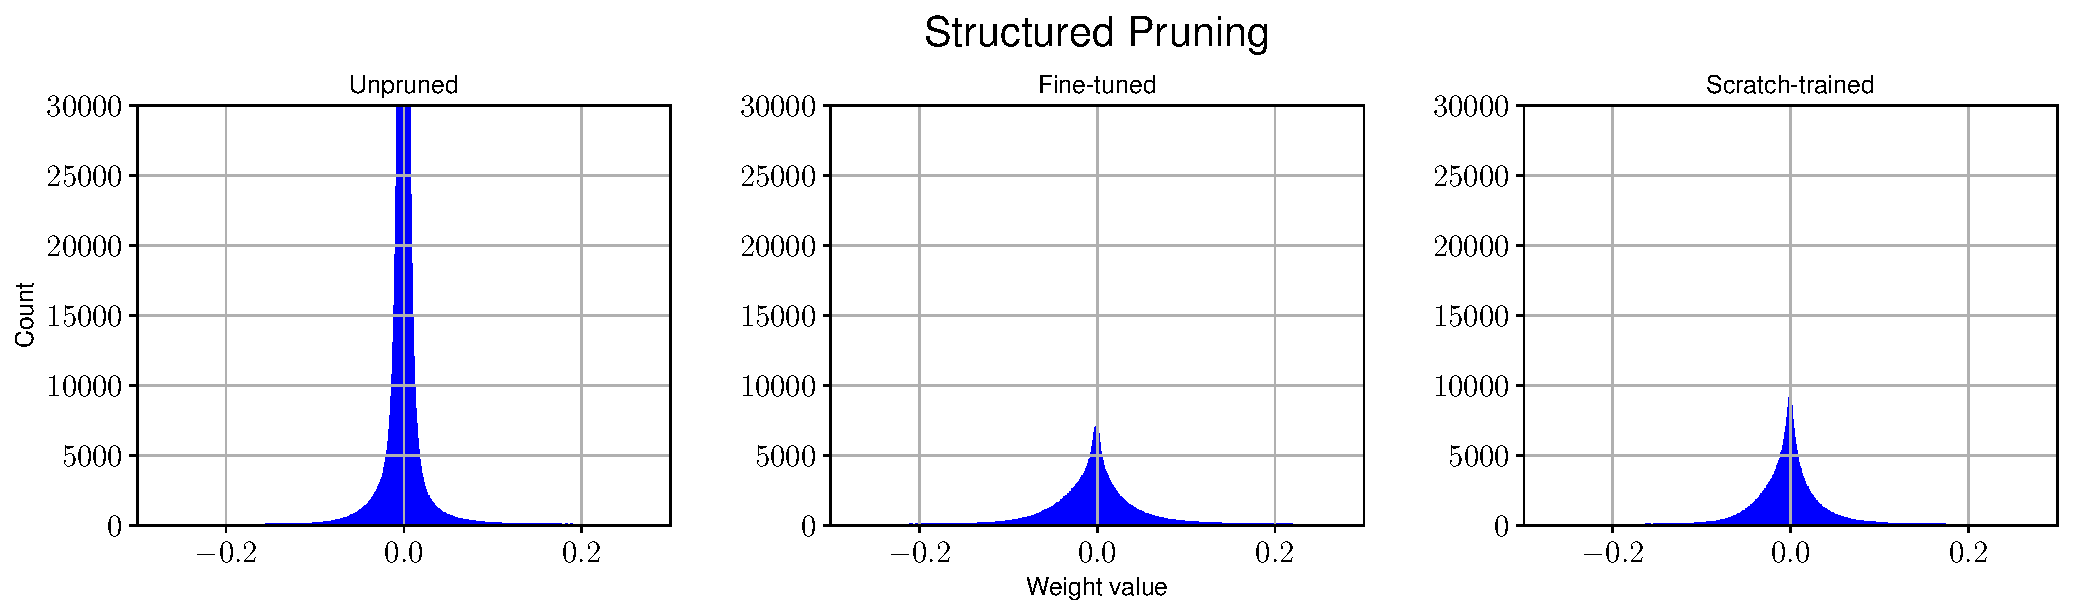
\includegraphics[width=\textwidth]{figures/channel-compressed.pdf}
 \label{arch-search-b1}
 \end{subfigure}
\end{minipage}
\begin{minipage}{\textwidth}
 \begin{subfigure}{\textwidth}
 \centering
% 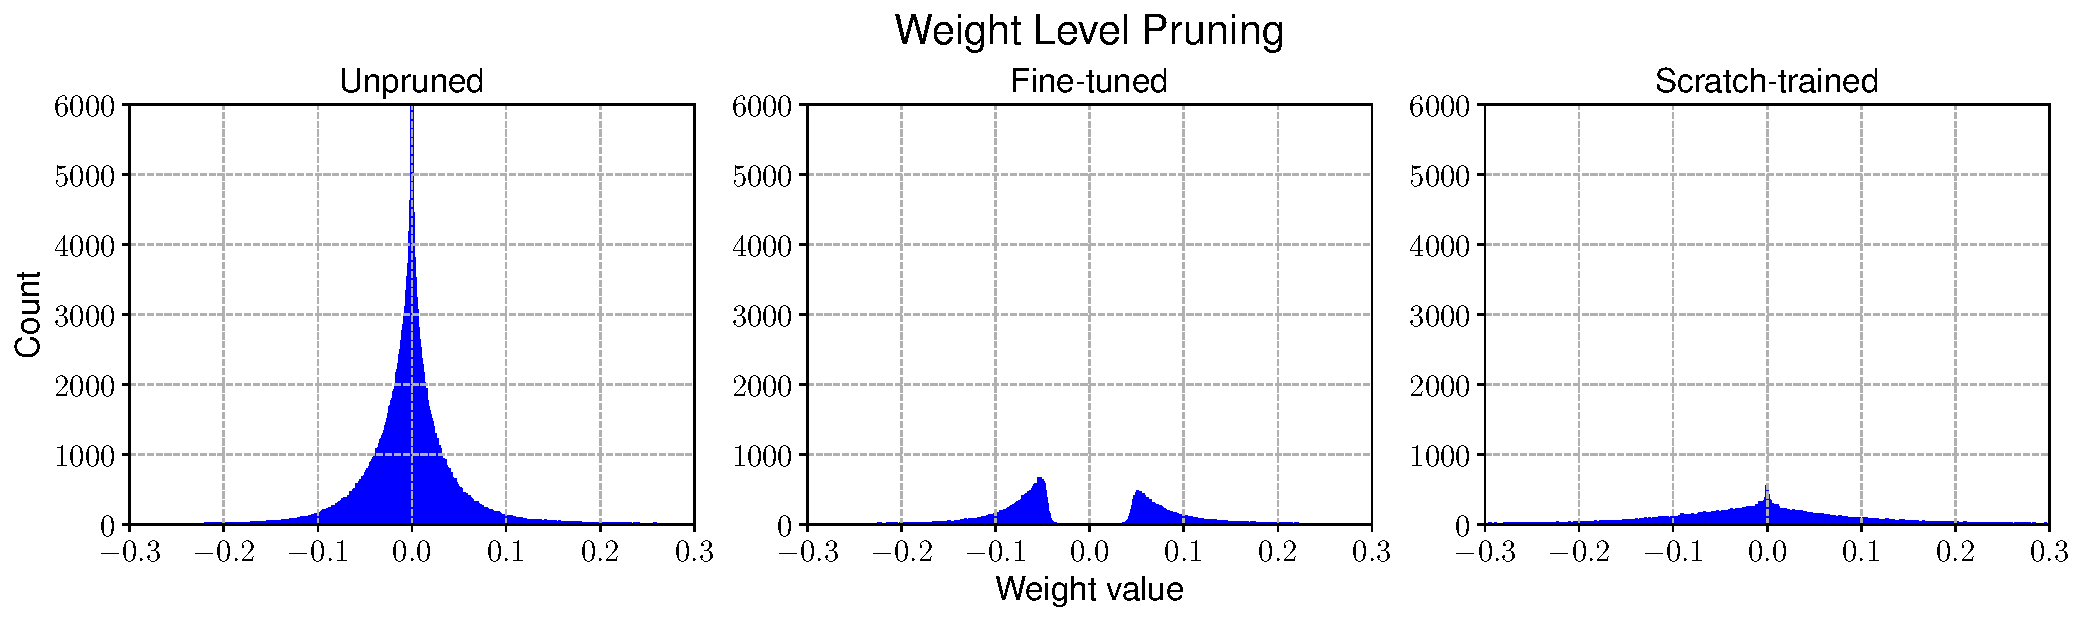
\includegraphics[width=\textwidth]{figures/weight-level-prune-dist-v2.pdf}
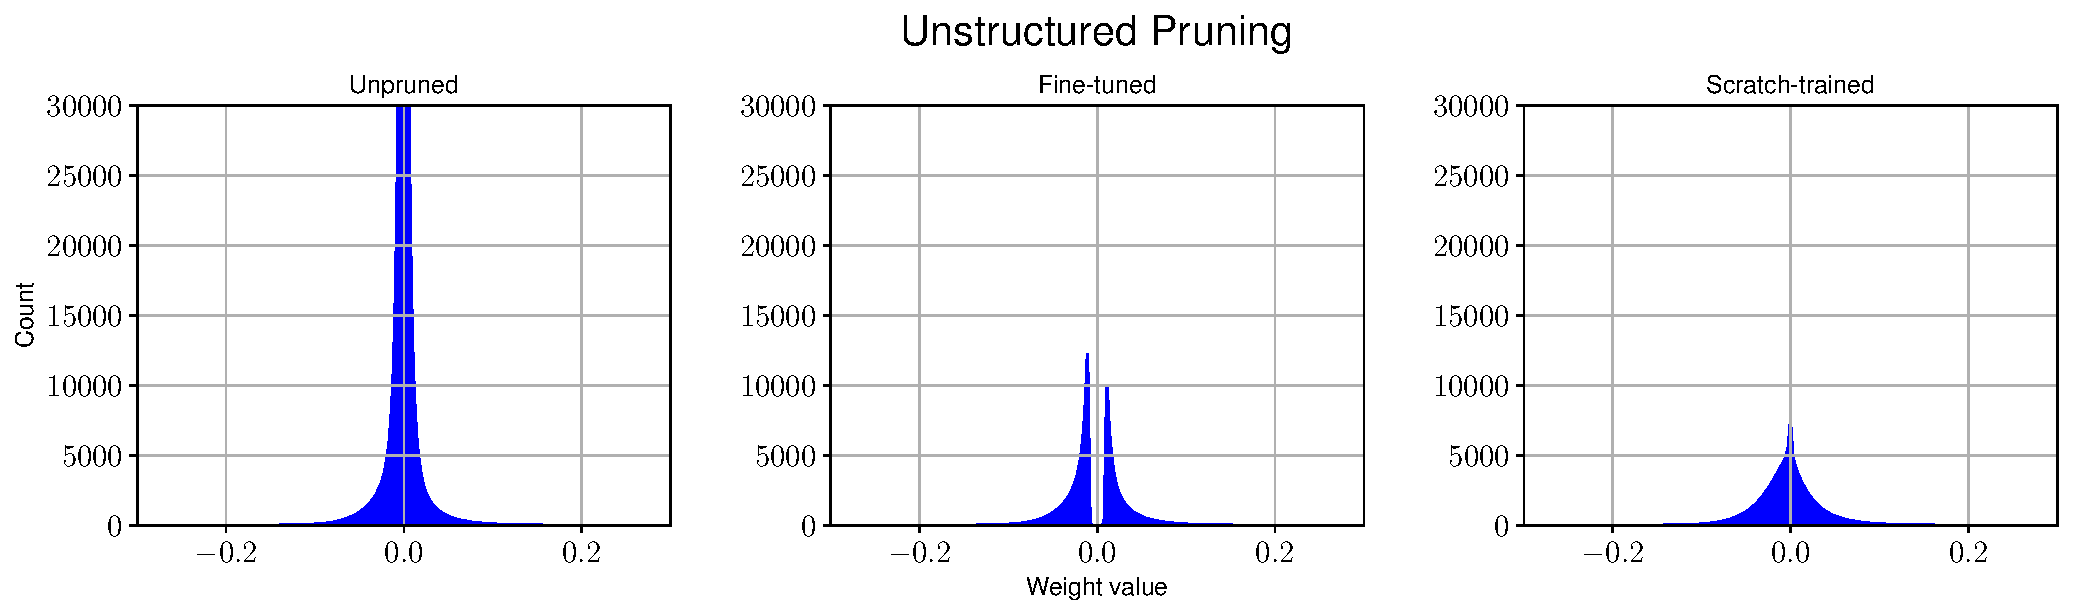
\includegraphics[width=\textwidth]{figures/weight-compressed.pdf}
%  \caption{}
 \label{arch-search-b}
 \end{subfigure}
\end{minipage}
    \vspace{-3ex}
    \caption{Weight distribution of convolutional layers for different pruning methods. We use VGG-16 and CIFAR-10 for this visualization. We compare the weight distribution of unpruned models,  fine-tuned models and scratch-trained models. \emph{Top}: Results for Network Slimming \citep{liu2017learning}. \emph{Bottom}: Results for unstructured pruning \citep{han2015learning}.}  
    \label{dist}
    \vspace{-1ex}
\end{figure}

Accompanying the discussion in \autoref{sec:unstructured}, we show the weight distribution of unpruned large models, fine-tuned pruned models and scratch-trained pruned models, for two pruning methods: (structured) Network Slimming~\citep{liu2017learning} and unstructured pruning~\citep{han2015learning}. We choose VGG-16 and CIFAR-10 for visualization and compare the weight distribution of unpruned models, fine-tuned models and scratch-trained models. For Network Slimming, the prune ratio is 50\%. For unstructured pruning, the prune ratio is 80\%. \autoref{dist} shows our result.  We can see that the weight distribution of fine-tuned models and scratch-trained pruned models are  different from the unpruned large models -- the weights that are close to zero are much fewer.  This seems to imply that there are less redundant structures in the found pruned architecture, and support the view of architecture learning for automatic pruning methods.

For unstructured pruning, the fine-tuned model also has significantly different weight distribution from the scratch-trained model -- it has nearly no close-to-zero values. This might be a potential reason why sometimes  models trained from scratch cannot achieve the accuracy of the fine-tuned models, as shown in \autoref{weight-level}.

\section{More Sparsity Patterns for Pruned Architectures}
\label{sec:additional}
% \vspace{-2ex}
In this section we provide the additional results on sparsity patterns for the pruned models, accompanying the discussions of ``More Analysis'' in Section \ref{sec:arch}.

\setlength{\tabcolsep}{5pt}
\renewcommand{\arraystretch}{1.2}
\begin{table}[!htbp]
% \vspace{-1ex}
\centering
\small
\begin{tabular}{c|ccccccc}
\hline
       & 10\%   & 20\%   & 30\%   & 40\%   & 50\%   & 60\%   & 70\%   \\ \hline
Stage 1 & 0.879 & 0.729 & 0.557 & 0.484 & 0.421 & 0.349 & 0.271 \\
Stage 2 & 0.959 & 0.863 & 0.754 & 0.651 & 0.537 & 0.428 & 0.320 \\
Stage 3 & 0.889 & 0.798 & 0.716 & 0.610 & 0.507 & 0.403 & 0.301 \\ \hline
\end{tabular}
\vspace{1ex}
  \caption{
      Sparsity patterns of PreResNet-164 pruned on CIFAR-10 by Network Slimming  shown in \autoref{arch-search-negative} (left) under different prune ratio. The top row denotes the total prune ratio. The values denote the ratio of channels to be kept. We can observe that for a certain prune ratio, the sparsity patterns are close to uniform (across stages).}
      \label{sparsity-5}
\end{table}


\setlength{\tabcolsep}{5pt}
\renewcommand{\arraystretch}{1.2}
\begin{table}[!htbp]
\centering
\small
\begin{tabular}{c|ccc|ccc|ccc}
\hline
                         & \multicolumn{3}{c|}{10\%} & \multicolumn{3}{c|}{50\%} & \multicolumn{3}{c}{90\%} \\ \hline
\multirow{3}{*}{Stage 1} & 0.905   & 0.905  & 0.909  & 0.530   & 0.561  & 0.538  & 0.129  & 0.171  & 0.133  \\
                         & 0.900   & 0.912  & 0.899  & 0.559   & 0.588  & 0.551  & 0.166  & 0.217  & 0.176  \\
                         & 0.903   & 0.913  & 0.902  & 0.532   & 0.563  & 0.547  & 0.142  & 0.172  & 0.163  \\ \hline
\multirow{3}{*}{Stage 2} & 0.906   & 0.911  & 0.906  & 0.485   & 0.523  & 0.503  & 0.073  & 0.102  & 0.085  \\
                         & 0.912   & 0.911  & 0.915  & 0.508   & 0.529  & 0.525  & 0.099  & 0.114  & 0.111  \\
                         & 0.911   & 0.916  & 0.912  & 0.502   & 0.529  & 0.519  & 0.080  & 0.113  & 0.096  \\ \hline
\multirow{3}{*}{Stage 3} & 0.901   & 0.904  & 0.900  & 0.454   & 0.475  & 0.454  & 0.043  & 0.059  & 0.048  \\
                         & 0.885   & 0.891  & 0.889  & 0.409   & 0.420  & 0.415  & 0.032  & 0.033  & 0.035  \\
                         & 0.898   & 0.903  & 0.902  & 0.450   & 0.468  & 0.458  & 0.042  & 0.055  & 0.046  \\ \hline
\end{tabular}
% }
\vspace{1ex}
  \caption{
      Average sparsity patterns of 3$\times$3 kernels of PreResNet-110 pruned on CIFAR-100 by unstructured pruning shown in \autoref{arch-search-negative} (middle) under different prune ratio. The top row denotes the total prune ratio. The values denote the ratio of weights to be kept. We can observe that for a certain prune ratio, the sparsity patterns are close to uniform (across stages).}
\label{sparsity-6}
\vspace{-2ex}
\end{table}


\setlength{\tabcolsep}{5pt}
\renewcommand{\arraystretch}{1.2}
\begin{table}[!htbp]
\centering
\small
% Please add the following required packages to your document preamble:
% \usepackage{multirow}
\begin{tabular}{c|ccc|ccc|ccl}
\hline
                         & \multicolumn{3}{c|}{10\%} & \multicolumn{3}{c|}{50\%} & \multicolumn{3}{c}{90\%} \\ \hline
\multirow{3}{*}{Stage 1} & 0.861   & 0.856  & 0.858  & 0.507   & 0.495  & 0.510  & 0.145  & 0.129  & 0.142  \\
                         & 0.843   & 0.844  & 0.851  & 0.484   & 0.486  & 0.479  & 0.123  & 0.115  & 0.126  \\
                         & 0.850   & 0.854  & 0.857  & 0.509   & 0.490  & 0.511  & 0.136  & 0.131  & 0.147  \\ \hline
\multirow{3}{*}{Stage 2} & 0.907   & 0.905  & 0.906  & 0.498   & 0.487  & 0.499  & 0.099  & 0.088  & 0.100  \\
                         & 0.892   & 0.888  & 0.892  & 0.442   & 0.427  & 0.444  & 0.064  & 0.043  & 0.065  \\
                         & 0.907   & 0.906  & 0.905  & 0.497   & 0.485  & 0.493  & 0.095  & 0.082  & 0.098  \\ \hline
\multirow{3}{*}{Stage 3} & 0.897   & 0.901  & 0.899  & 0.470   & 0.475  & 0.472  & 0.060  & 0.060  & 0.064  \\
                         & 0.888   & 0.890  & 0.889  & 0.433   & 0.437  & 0.435  & 0.040  & 0.040  & 0.042  \\
                         & 0.898   & 0.900  & 0.899  & 0.473   & 0.477  & 0.473  & 0.060  & 0.061  & 0.063  \\ \hline
\end{tabular}
% }
\vspace{1ex}
  \caption{
      Average sparsity patterns of 3$\times$3 kernels of DenseNet-40 pruned on CIFAR-100 by unstructured pruning shown in \autoref{arch-search-negative} (right) under different prune ratio. The top row denotes the total prune ratio. The values denote the ratio of weights to be kept. We can observe that for a certain prune ratio, the sparsity patterns are close to uniform (across stages).}
\label{sparsity-8}
 \vspace{-2ex}
\end{table}

\setlength{\tabcolsep}{5pt}
\renewcommand{\arraystretch}{1.2}
\begin{table}[!htbp]
\centering
\small
% \resizebox{1.0\textwidth}{!}{
\begin{tabular}{c|cccccc}
\hline
      & 10\%   & 20\%   & 30\%   & 40\%   & 50\%   & 60\%   \\ \hline
Stage 1 & 0.969 & 0.914 & 0.883 & 0.875 & 0.844 &
0.836 \\
Stage 2 & 1.000 & 1.000 & 1.000 & 1.000 & 1.000 &
1.000 \\
Stage 3 & 0.991 & 0.975 & 0.966 & 0.957 & 0.947 & 0.947 \\
Stage 4 & 0.861 & 0.718 & 0.575 & 0.446 & 0.312 & 0.258 \\
Stage 5 & 0.871 & 0.751 & 0.626 & 0.486 & 0.352 & 0.132 \\ \hline
\end{tabular}
% }
    \vspace{1ex}
    \caption{
      Sparsity patterns of VGG-16 pruned on CIFAR-10 by Network Slimming shown in Figure~\ref{arch-search} (left) under different prune ratio. The top row denotes the total prune ratio. The values denote the ratio of channels to be kept. For each prune ratio, the latter stages tend to have more redundancy than earlier stages.}
     \label{sparsity-2}
     \vspace{-2ex}
\end{table}